%docmentclass
\documentclass[twoside,12pt]{article}

\usepackage{minted}

\usepackage{fancyhdr}


%code blocks
\usepackage{listings}

%figures
\usepackage{tikz}
\usetikzlibrary{matrix,positioning,shapes,backgrounds}
\usepackage{pgf-pie}

%for figures 
\usepackage{float}

%displaying last page number
\usepackage{lastpage}

%package declarations
\usepackage{hyperref}

% palatino clone as font
\usepackage[sc]{mathpazo}   

% Palatino needs more leading (space between lines)
\linespread{1.05}

\usepackage{tabularx}

% font encoding done right
\usepackage[T1]{fontenc}

% 
\usepackage{caption}
\usepackage{subcaption}

\usepackage{booktabs}

% input encoding done right
\usepackage[utf8]{inputenc} 

% finnish
\usepackage[finnish]{babel} 

% apacite is the bibliography style
\usepackage{apacite}        

% correct margins
\usepackage[top=3cm, bottom=2.5cm, left=3cm, right=3cm]{geometry} 

\usepackage{graphicx}       % we need graphics
\usepackage{tocloft}        % table of contents package 
\usepackage{afterpage}      % package to enable commands after pages
\usepackage{color}          % colors enabled for comments 

%\usepackage{pgf-pie}

\newcommand                 % command for making red emphasized comments for reader.
    \comment[1]{
        \color{blue}
        \emph{#1}
        \color{black}
        }

% SETTINGS

\setcounter{tocdepth}{2}    % show only sections

\bibliographystyle{apacite} % apacite päälle

\AtBeginDocument{                                               % hienosäätöä englanti -> suomi
    %\renewcommand{\BCBT}{}
    \renewcommand{\BOthers}[1]{ym.\hbox{}}                      % et. al -> ym.
    \renewcommand{\BOthersPeriod}[1]{ym.\hbox{}}                % et. al -> ym.
    \renewcommand{\refname}{LÄHTEET}                            % viitteet -> lähteet
    \renewcommand{\cftsecleader}{\cftdotfill{\cftsecdotsep}}    % pisteet @ ToC
    \renewcommand\cftsecdotsep{\cftdot}                         % pisteet @ ToC
    \renewcommand\cftsubsecdotsep{\cftdot}                      % pisteet @ ToC
    \renewcommand\listfigurename{\normalsize{KUVIOT}}
    \renewcommand\listtablename{\normalsize{TAULUKOT}}
    \renewcommand{\cftfigleader}{\cftdotfill{\cftsecdotsep}}
    \renewcommand{\cfttableader}{\cftdotfill{\cftsecdotsep}}
    }
    


\addto\captionsfinnish{%
  \renewcommand{\figurename}{Kuvio}%
  %\renewcommand{\contentsname}{Table of Contents}%
}

\let\oldsection\section % newpage after section

%content section
\newcommand{\jyusection}[1]{
    \newpage
    \vspace*{4cm}
    \section{#1}
    }
        
%sections in abstract dosn't take vertical space, only new page.
\newcommand{
    \abstractsection}[1]{ 
      \newpage
      \oldsection*{#1}
      \cftaddtitleline{toc}{section}{#1}{}
    }
    
%attachments also in new page, no vfill.
\newcommand{\attachmentsection}[1]{
    \newpage
    \oldsection*{#1}
    \addcontentsline{toc}{section}{#1}
    }
    

%bibliography redefined without top margin
\newcommand{\jyubibliography}{
    \newpage
    \bibliography
    }
    
% suppress underfull badness warnings
\hbadness = 10000


    
\begin{document}

\addtocontents{toc}{\protect\renewcommand{\protect\cftsecleader}{\hfill}}

%frontcover
\begin{center}
    \vspace*{5cm}
    \normalsize{Tuomas-Matti Soikkeli} \\
    \large{NoSQL-tietokannat: perusominaisuudet ja luokittelu} \\
        \vfill{}
    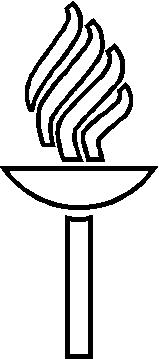
\includegraphics[width=0.1\textwidth]{images/jyu.jpg} \\
    \large{JYVÄSKYLÄN YLIOPISTO \\
    TIETOJENKÄSITITTELYTIETEIDEN LAITOS \\
    2015}
\end{center} 

%remove page numbering from front page
\thispagestyle{empty}

%Finnish abstract
\abstractsection{TIIVISTELMÄ}

%remove page numbering from abstract
\thispagestyle{empty}

%\addcontentsline{toc}{section}{TIIVISTELMÄ}
Soikkeli, Tuomas-Matti \hfill \\
Kandidaatintutkielma \hfill \\
Jyväskylä: Jyväskylän yliopisto, 2014, \pageref{LastPage} s. \hfill \\
Tietojärjestelmätiede \hfill \\
Ohjaaja: Leppänen, Mauri \hfill \\ \\
{\color{red}
Tässä tutkielmassa tutkitaan kirjallisuuskatsauksen avulla miten NoSQL-tietokantoja voidaan luokitella ja mitkä ovat niiden käyttökohteet. Toiseksi tutkitaan miten NoSQL-tietokannat ovat kehittyneet ja minkälaisia ominaispiirteiltä niillä on. Samalla tutustutaan miten NoSQ-tietokannat eroavat perinteisistä relaatiotietokannoista ja voidaanko relaatiotietokannat korvata NoSQL-tietokannoilla. Lisäksi tutkitaan NoSQL-tietokantoihin kohdistunutta krittiikiä. Lopuksi tässä tutkielmassa NoSQL-tietokannat luokitellaan neljään ryhmään: avain-arvopari-varastot, dokumenttivarastot, sarakepohjaiset tietokannat ja verkkotietokannat. Jokaisen tietomallin kohdalla esitellään tarkemmin tietomallin piirteet ja käyttökohteet sekä havainnollistetaan tietomallia esimerkein.} \hfill \\ \\
Asiasanat: NoSQL, tietokanta, ei-relaationaalinen \hfill
\newpage

%English Abstract
\abstractsection{ABSTRACT}

%remove page numbering
\thispagestyle{empty}

Soikkeli, Tuomas-Matti \hfill \\
Candidate's thesis  \hfill \\
Jyväskylä: University of Jyväskylä, 2014, \pageref{LastPage} p. \hfill \\
Information Systems, Candidates Thesis \hfill \\
Supervisor(s): Leppänen, Mauri \hfill \\ \\

{\color{red}In this candidate's thesis NoSQL-databases are researched to categorize and identify the most common usecases for them. Secondly the author researches how NoSQL-databases are evolved and what are their main properties. At the same time, NoSQL-databases are compared how they differ from ordinary relational database management systems and are these relational databases replaceable with NoSQL-databases. Moreover we study the critque that the NoSQL faces. Finally, NoSQL-databases are divided into four groups: key-value stores, document stores, column based databases and graph databases. In each data model we study the common properties of particular data model and we explore the use cases for these data models. This is done by providing real-world examples. \hfill \\ \\}
Keywords: NoSQL, database, non-relational \hfill 
\newpage

%list of figures and list of tables
\listoffigures
\cftaddtitleline{toc}{section}{KUVIOT}{}%
\listoftables
\cftaddtitleline{toc}{section}{TAULUKOT}{}%
% remove page numbering (has to be last, \tableofcontents overrides)
\thispagestyle{empty}
\newpage

%ToC
\tableofcontents 
\cftaddtitleline{toc}{section}{SISÄLLYS}{}%
% remove page numbering (has to be last, \tableofcontents overrides)
\thispagestyle{empty}
\newpage

% add dotted line to top-level TOC-entries
\addtocontents{toc}{\protect\renewcommand{\protect\cftsecleader}{\protect\cftdotfill{\protect\cftsecdotsep}}}

%add page numberin on top
\fancyhf{}
\renewcommand{\headrulewidth}{0pt}
\fancyhead[LE,RO]{\thepage}
\pagestyle{fancy}

%contents
\jyusection{ESIPUHE}
Tämä tutkielma on tehty \LaTeX-ladontajärjestelmällä, jota suosittelen lämpimästi kaikille tutkielman kirjoittajille. Tutkimussuunnitelman kirjoittamisen aikaan Jyväskylän Yliopiston Tietojärjestelmätieteiden opiskelijoille oli tarjolla vain Microsoft Word -dokumenttipohja, jonka moninaiset ongelmat saivat minut harkitsemaan muita vaihtoehtoja. Tuloksena syntyi dokumenttipohja, jonka olen julkaissut avoimena lähdekoodina. Varoituksen sanana voin sanoa, että siirtymä tavanomaisista tekstinkäsittelyohjelmista ei ole helppo. Opettelu vaatii runsaasti aikaa, kuten tämän tutkielman tekeminen osoitti.

Päädyin käyttämään tekstin ja koodin muokkamiseen web-pohjaista, sekä ilmaista ShareLatex (http://www.sharelatex.com) -palvelua. ShareLatex-editori ja -kääntäjä suoraviivaistaa monia \LaTeX:n monimutkaisuuksia. Lähdekoodi on saatavilla kokonaisuudessaan osoitteesta: https://github.com/t-my/tuomas-soikkeli-candidates-thesis


{\color{red}
\jyusection{JOHDANTO}

Useat suuret organisaatiot ja yritykset kuten esimerkiksi Google, Amazon ja LinkedIn tallentavat mittavia määriä dataa jatkokäyttöä ja analyysiä varten. Tyypillisesti tiedon tallentamiseen on käytetty SQL-tietokantoja, joihin tieto tallennetaan rakenteelliseen muotoon relaatiomallin mukaan. Rakenteellisen tiedon tallennus ja hakeminen ovat kalliita ja aikaavieviä operaatioita. Siten datamäärien kasvaessa eksponentiaalisesti on kehitetty ei-relaationaalisia tietokantajärjestelmiä. Näitä järjestelmiä kutsutaan NoSQL -tietokannoiksi. \cite{leavitt2010will, pokorny2013nosql}

2000-luvulta alkaen on kehitetty NoSQL-tietokantoja perinteisten relaatiotietokantojen rinnalle. 

Näitä tietomalleja ovat esimerkiksi avain-arvo-pari\-varastot, dokumenttivarastot, sarakepohjaiset tietokannat ja verkkotietokannat. Myös muita tietomalleja käyttäviä järjestelmiä on runsaasti, mutta tässä tutkielmassa keskitytään näiden neljän tietomallin tutkimiseen. \cite{cattell2011scalable}


NoSQL-tietokantojen nuoren iän myötä NoSQL-tietokannoista ei ole kattavaa tutkimustietoa. Tässä tutkielmassa tutkitaan näitä epäselvyyksiä seuraavien tutkimuskysymysten avulla:

\begin{itemize}

\item Miten NoSQL-tietokantoja voidaan luokitella?

\item Miten NoSQL-tietokannat eroavat relaatiomalliin perustuvista tietokannoista?

\item Mihin käyttötarkoitukseen NoSQL-tietokantoja voidaan käyttää?

\item Voidaanko NoSQL-tietokannoilla korvata relaatiotietokannat?

\end{itemize}

Tämä tutkielma selvittää kirjallisuuskatsauksen avulla aluksi NoSQL-tieto\-kantojen kehitykseen ja historiaan liittyviä seikkoja. Sen jälkeen tutkitaan miksi NoSQL-tieto\-kannat ovat kasvattaneet suosiotaan, miten NoSQL-tietokantoja voidaan luokitella sekä mitä käyttökohteita NoSQL-tietokannoilla on. Samalla selvitetään miten nämä tietokannat eroavat relaatiomallista ja sen tiedon manipulointiin liittyvästä SQL-kielestä. 

Tämän tutkimuksen avulla lukijaa saa selvän kuvan tietokantojen teoriapohjasta, NoSQL-tietokantojen tyypillisistä käyttökohteista sekä tavanomaisista ominaisuuksista.

Tämä tutkimus jakaantuu kolmeen sisältölukuun. Ensimmäisessä sisältöluvussa tutustutaan NoSQL-tietokantojen kehittymiseen johtaneisiin seikkioihin eli historiaan. Tämän lisäksi ensimmäisessä kappalessa käydään läpi relaatiotietkantojen ja NoSQL-tietokantojen toiminnan teoriaa ja ominaisuuksia. Toisessa kappalessa määritelmän jälkeen käydään läpi NoSQL-tietokantojen keskisimmät ominaisuudet ja yleisimmät määrittelevät tekijät. Toisen kappaleen lopussa käsitellään myös krittiikkiä aiheeseen liittyen.Kolmannessa kappaleessa esitellään aluksi luokittu, jonka jälkeen käydään läpi tietokantasovelluksia tietomalleittain.
}

\jyusection{NOSQL-TIETOKANTOJEN TAUSTA} 

Tässä luvussa kuvataan NoSQL-tietokantojen kehittämiseen johtaneita syitä. Aluksi kerrotaan lyhyest relaatiotietokannoista ja SQL:stä. Toiseksi käsitellään relaatiotietokannoille olennaisia ACID-ominaisuuksia. Kolmanneksi kerrotaan, kuinka tiedon valtava massa verkkoliikenteessä on muuttanut tiedonkäsittelyn ja tallentamisen vaatimuksia. Lopuksi esitellään CAP-teoreema ja sen pohjalta kehitetty BASE-oikeellisuusmalli, joka mahdollistaa tiedon tehokkaan tallentamisen ja käsittelyn hajautetussa ympäristössä.

\subsection{Relaatiotietokannat ja SQL}

Edgar Codd (1970) esitti tietomallin, jolla voidaan (silloisia valtamalleja, verkkomallia ja hierarkkista mallia) yksinkertaisemmalla ja fyysistä rakenteista riippumattomalla tavalla jäsentää tallentavaa tietoa. Tämä malli sai nopeasti suosiota ja johti useiden tutkimusprojektien \cite{chamberlin1974sequel} kautta SQL-kyselykielen (engl. Structured Query Language) syntyyn \cite[s.~8-10]{melton1993understanding}. SQL-kielen standardoinnin \cite[s.~3]{melton1993understanding} jälkeen sitä onkin käytetty laajamittaisesti tiedon tallentamiseen. SQL:ään perustuvat relaatiotietokannat ovat tämän hetken suosituinpia tietokannan hallintajärjestelmiä.

Relaatiomallissa (kuvio \ref{relaatiomalli}) tieto tallennetaan tauluihin, joka kostuu riveistä ja riveillä olevista arvoista. Taulut voidaan linkittää toisiinsa moninaisten avainarvojen avulla. 

\begin{figure}[H]
\begin{center}

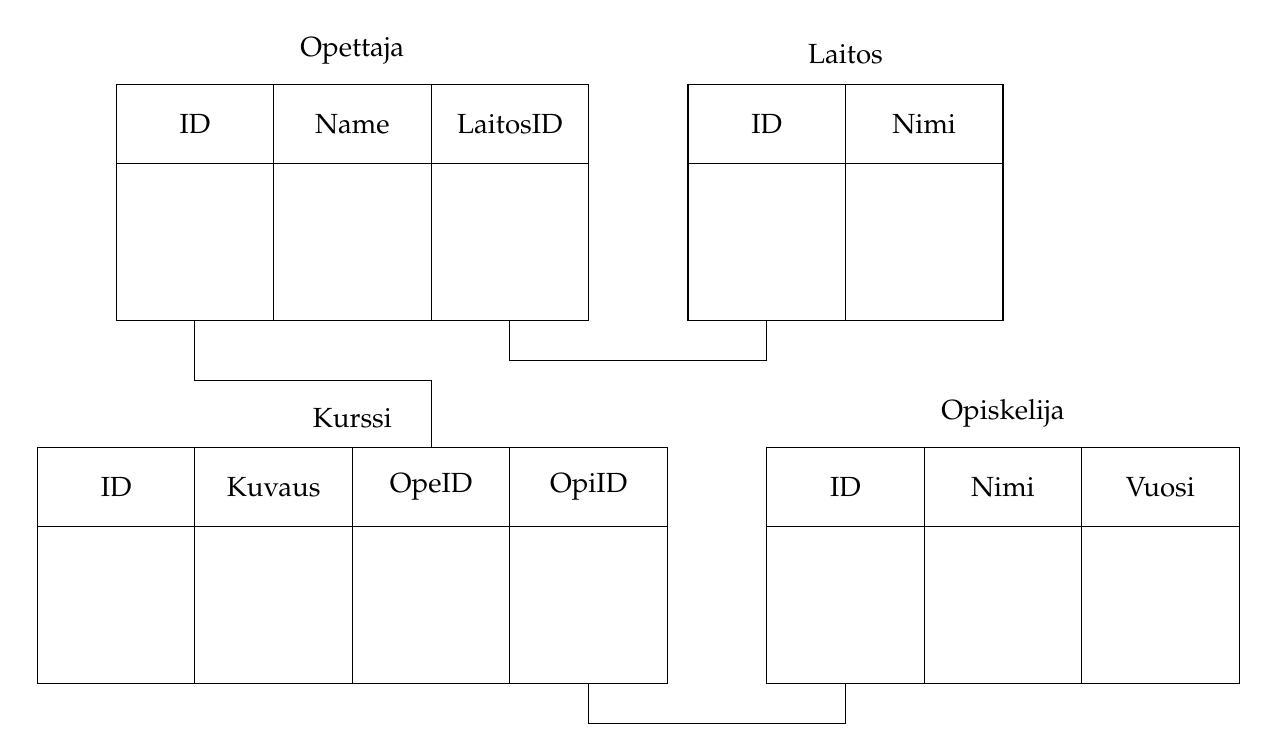
\begin{tikzpicture}[
table/.style={matrix of nodes, nodes in empty cells, column sep=-\pgflinewidth, row sep=-\pgflinewidth, nodes={draw,anchor=center,minimum width=2cm,minimum height=2cm}, row 1/.style={nodes={minimum height=1cm}}}]

\matrix(Laitos) [table, label=above:Laitos] {
    ID & Nimi \\ & \\};

\matrix(Opettaja) [table, label=above:Opettaja, left=1cm of Laitos] {
    ID & Name & LaitosID \\ & & \\};

\matrix(Kurssi) [table, label=above:Kurssi, below=1.35cm of Opettaja] {
    ID & Kuvaus & OpeID & OpiID \\ & & & \\};

\matrix(Opiskelija) [table, label=above:Opiskelija, right=1cm of Kurssi] {
    ID & Nimi & Vuosi \\ & & \\};

\draw (Laitos-2-1.south)--++(0,-.5)-|(Opettaja-2-3.south);
\draw (Opettaja-2-1.south)--++(0,-.75)-|(Kurssi-1-3.north);
\draw (Kurssi-2-4.south)--++(0,-.5)-|(Opiskelija-2-1.south);

\end{tikzpicture}

\caption[RELAATIOMALLI]{Tauluihin ja riveihin perustuva esimerkki relaatiomallista}
\label{relaatiomalli}
\end{center}
\end{figure}

\subsection{ACID}
Tietokanta sisältää suuren määrän tietoja, joita monet ohjelmat voivat samaan aikaa hakea ja päivittää. Jotta voidaan varmistaa se, etteivät samaan tietoon kohdistuvat operaatiot samaan aikaan suoritetteuina tuota ongelmia, tarvitaan jokin samanaikaisten tapahtumien hallintamekanismi. Andreas Reuter ja Theo Härder julkaisivat vuonna 1983 artikkelin "Principles of Transaction-Oriented Databasse Recovery", joissa he aiempiin tutkimuksiin pohjautuen \cite{gray1981transaction,international1979notes} määrittelivät termin ACID, joka on lyhenne sanoista Atomicity, Consistency, Isolation ja Durability. Vastaavat suomenkieliset termit ovat atomisiuus, eheys, eristyneisyys ja pysyvyys. 

ACID tarkoittaa joukkoa ominaisuuksia, jotka takaavat tietokannan tapahtumien suorituksen luotettavuuden niin, että jokaisen tapahtuman suorituksen jälkeen pystytään varmistumaan, että halutut operaatiot ovat oikein suoritettu. Esimerkiksi siirrettäessä rahaa toisen käyttäjän tilille on varmistettava, että tapahtuma, jolla nostetaan rahaa toiselta tililtä ja pannaan vastaava summa toiselle tilille, on todella tapahtunut alusta loppuun. Mikäli tapahtuman suorituksen aikana sattuu järjestelmän kaatuminen, on palattava alkuperäiseen järjestelmän tilaan. Seuraavaksi annettaan edellä mainituille termeille lyhyet määritelmät \cite{haerder1983principles}:


\newpage

\begin{itemize}

\item \textbf{Atomisuus:} Tapahtuman aikana suoritetaan joko kaikki tietokantaoperaatiot tai ei ainuttakaan. Täten jos yksi osa tapahtumasta epäonnistuu, koko transaktio epäonnistuu.

\item \textbf{Eheys:} Tapahtuman tulee jatkuvasti täyttää kaikki eheyssäännöt. Tapahtuma ei riko näitä sääntöjä, joten tietokanta pysyy yhtenäisessä tilassa tapahtuman suorituksen aikana. 

\item \textbf{Eristyneisyys:} Tapahtuma tulee voida suorittaan ikään kuin muita samanaikaisia tapahtumia ei olisikaan. Toisin sanoen muiden tapahtumien ei tule vaikuttaa sen suorittamiseen. 

\item \textbf{Pysyvyys:} Vahvistetun (commited) tapahtuman tekemät muutokset tietokannassa ovat lopullisia. Niihin eivät vaikuta mahdolliset virheet tai häiriöt.

\end{itemize}

ACID-ominaisuuksien varaan on relaatiotietokannoille kehitetty mekanismeja (esim. lukitusprotokollat, toipuminen), joilla pyritään turvaamaan tietokannan eheys kaikissa olosuhteissa. Seuraavassa alaluvussa esitellään tiedon määrän kasvaminen ja sen aiheuttamat kustannukset ACID-ominaisuudet täyttävässä järjestelmässä. 

\subsection{Tiedon valtava massa}

Internetin kehityksen myötä tietokantojen vaatimukset ovat muuttuneet. \citeA{manyika2011big} esitti tutkimuksessaan, että alle tuhannen työntekijän yrityksillä on keskimäärin 3,8 petatavua dataa tallennettuna ja vuotuinen datan määrän kasvus on neljäkymmentä prosenttia. Tätä tiedon jatkuvasti kasvavaa tulvaa kutsutaan massadataksi (engl. Big Data).

Näin ollen tarvitaan erittäin tehokkaita järjestelmiä, jotka pystyvät prosessoimaan suuria tietomääriä \cite{han2011survey}. Näihin vaatimuksiin perinteiset SQL-tietokannat eivät pysty enää vastaamaan kunnolla. Koska SQL-tietokannat käsittelevät dataa ACID-ominaisuuksia noudattaen\cite{pokorny2013nosql}, jokaisen yksinkertaisen solun ja rivin tallentamisen yhteydessä pitää varmistua tietokannan tapahtumien luotettavuudesta. Tämä hidastaa merkittävästi käsittelyn nopeutta, kun dataa on runsaasti. Yhtäaikaisten tapahtumien luotettava käsittely ei ole enää mahdollista, sillä tiedon tallentamisen ja käsittelyn kustannukset alkavat kasvaa eksponentiaalisesti käsiteltävän tietomäärän kasvaessa suureksi.

Tietokantajärjestelmille on muodostunut uusi haaste. Tietoa on yksikertaisesti liikaa, jotta sitä voitaisiin käsitellä käyttäen ACID-ominaisuuksia. Seuraavaksi esitellään teoreema, joka auttaa väljentämään tietokannalle asetettuja vaatimuksia.

\newpage

\subsection{CAP-teoreema ja BASE-oikeellisuusmalli}

Eric Brewer esitti vuonna 2000 \cite{brewer} kuviossa 2 esitetyn CAP-teoreeman, jota kutsutaan myös Brewerin teoreemaksi. CAP-teoreeman mukaan, on olemassa kolme ominaisuutta, jotka vaikuttavat hajautetun järjestelmän suunnittelun, toteutukseen ja käyttöönottoon. Nämä ominaisuudet ovat eheys, saatavuus ja pirstoutumisen sietokyky eli CAP (engl. consistency, availability, partition tolerance). 

Eheys (consistency) tarkoittaa, että tietokannan tosinteiden (replicates) tulee olla eheitä, jolloin hajautetun järjestelmän solmut näkevät kunkin tiedon samanlaisena. Saatavuus (availability) tarkoittaa, että palvelu (tietyn tiedon lukeminen tai kirjoittaminen) on saatavissa silloin, kun sitä tarvitaan. Pirstoutumisen sietokyky (partition tolerance) tarkoittaa, että verkon pirstoutuessa tiedonkäsittelyn tulee jatkua edelleen solmuissa \cite[s. 10]{celko2013joe}.

% CAP-theorem
\begin{figure}[H]
\begin{center}
    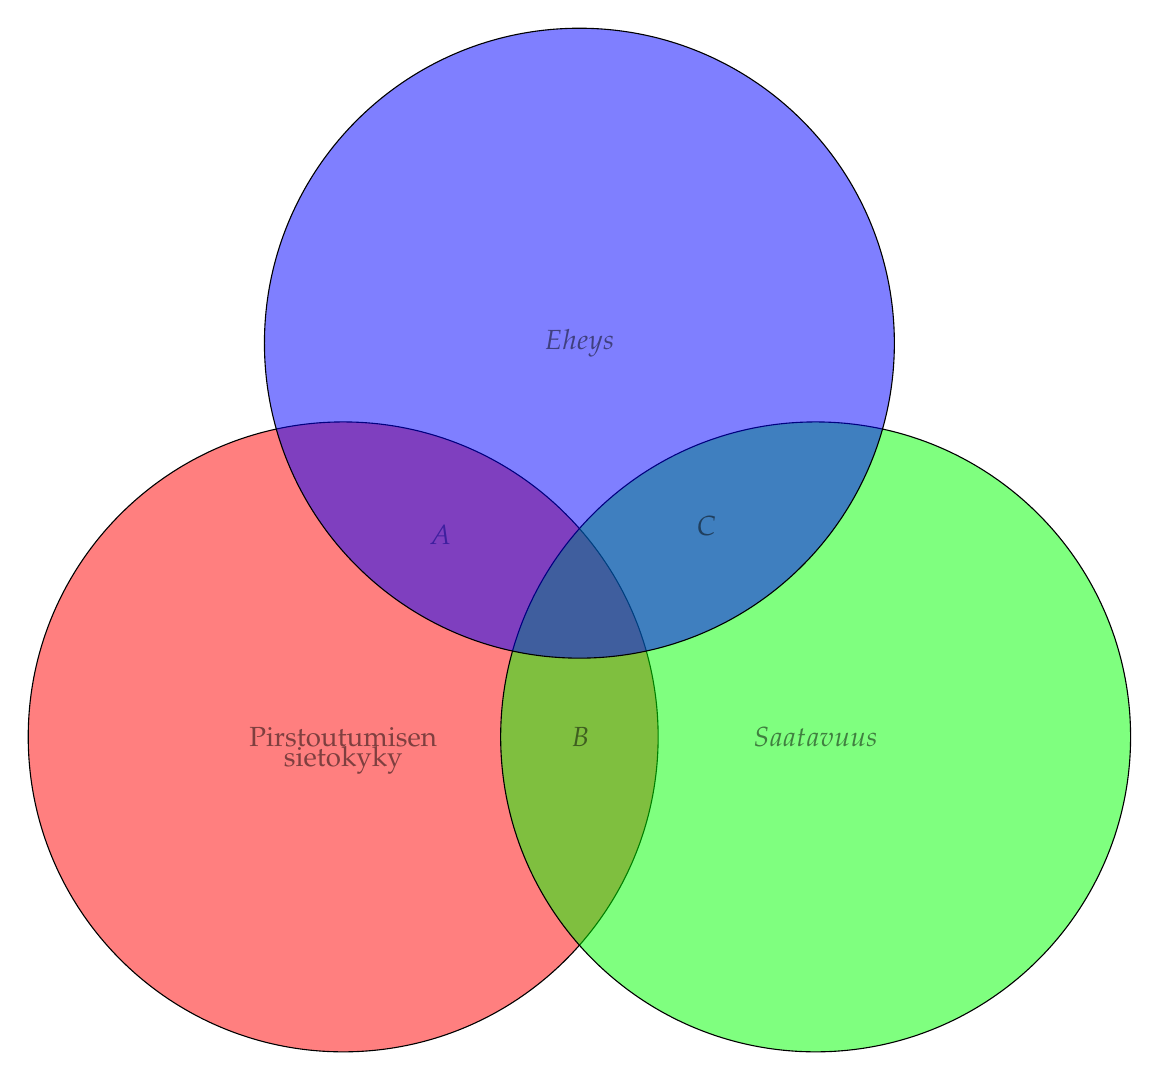
\begin{tikzpicture}
    \begin{scope}[fill opacity=0.5]
        
        \draw
        [fill=red](-3,0) 
        circle (4cm) 
            node {Pirstoutumisen}
            node[below] {sietokyky}
            node[above right=2.5cm, xshift=-0.8cm,yshift=0.55cm] {$A$};
        \draw
        [fill=green]
        (3,0) circle (4cm) 
            node {$Saatavuus$}
            node[left=2.75cm] {$B$};
        \draw
        [fill=blue](0,5) 
        circle (4cm) 
            node {$Eheys$} 
            node[below right=2.5cm,xshift=-0.4cm,yshift=-0.3cm] {$C$};
            
    \end{scope}
    \end{tikzpicture}
    \caption[CAP-TEOREEMA]{Hajautetun järjestelmän kolme ominaisuutta: CAP-teoreema (Brewerin teoreema)}
    \label{cap}
\end{center}
\end{figure}


\noindent Brewerin mukaan ei ole mahdollista taata jokaisen kolmen vaatimuksen toimivuutta. Tämä tulee ottaa huomioon järjestelmän suunnittelussa. Jos näin ei tehdä, voi lopputuloksena olla, että jokainen esitetty ominaisuus järjestelmässä rikkoutuu yhtä aikaa. \citeA{gilbert2002brewer} todistivat Brewerin olleen oikeassa ja tätä pidetäänkin yleisesti hyväksyttävänä lähestymistapana tietokantojen tarkasteluun \cite<mm.>{vogels2009eventually, cattell2011scalable, pokorny2013nosql}.

Tietokannan valinnassa tulee ottaa huomioon CAP-teoreemassa esitellyt kolme ominaisuutta. Yhdestä niistä on luovuttava. Saatavuuden ja eheyden omaavat tietokannat (C) ovat usein perinteisiä relaatiotietokantoja. Data on aina saatavilla ja tiedon eheys taataan erilaisten tekniikoiden, kuten viite-eheyden avulla. Näillä tietokannoilla on kuitenkin hankaluuksia verkon pirstaloituessa. Eheyttä ja pirstoutumisen sietokykyä tarjoavat (A) tietokannat puolestaan eivät voi taata tiedon saatavuutta. Saatavuutta ja pirstoutumisen sietokyvykä tarjoavat tietokannat (B) saavuttavat lopulta oikeellisen tiedon. \cite{hurst2010visual}

BASE-oikeellisusmallin avulla pyritään takaamaan hajautetuille jär\-jes\-tel\-mil\-le\linebreak mahdollisimman korkea saatavuus ja tehokkuus. BASE-mallin esitti \citeA{vogels2009eventually}, ja se nimi on lyhenne sanoista Basically Available, Soft state ja Eventual Consistency. Vastaavat suomenkieliset termit ovat: periaattessa käytettävissä, ei aina oikeellinen ja lopulta oikeellinen. Periaattessa käytettävissä tarkoittaa, että tiedon halutaan olevan käytettävissä aina vaikkei se olisikaan ajan tasalla. Ei aina oikeellinen tarkoittaa, että haettu tieto ei ole välttämättä oikea johtuen eri solmujen eri tiloista. Lopulta oikeellinen tarkoittaa, että vaikka tiedot eivät ole joka hetki eheitä, järjestelmä pitää huolen, että ne tulevat eheiksi jollakin aikavälillä. Se minkä ajan kulutta näin tapahtuu, riippuu järjestelmän muista ominaisuuksista kuten senhetkisen kuorman määrästä. \cite[s.11]{celko2013joe}


BASE-ominaisuudet tarkoittavat käytännössä, että tietokantajärjestelmä saattaa palauttaa vanhentuneen arvon, jonka tulisi jo olla päivittynyt. Tämä ei aina ole kuitenkaan ongelmallista. Esimerkiksi sosiaalisen median datan ei tarvitse olla reaaliaikaisesti saatavilla, vaan riittää että tieto leviää palvelimien välillä kohtuullisen ajan kuluessa. Tietokantaa suuniteltaessa ACID -ominaisuuksien sijasta BASE  -oikeellisuusmallin valitseminen antaa mahdollisuuden kehittää erittäin tehokkaita tietokantajärjestelmiä, koska tiedon oikeellisuudesta ei tarvitse varmistua välittömästi \cite{Bailis:2013:ECT:2460276.2462076}.

\jyusection{NOSQL-TIETOKANNAT}

Tässä luvussa esitellän NoSQL-tietokantoja, jotka pyrkivät ratkaisemaan jatkuvasti kasvavan tiedon määrän luomat haasteet. Aluksi määritellään NoSQL-käsite. Toiseksi esitellään NoSQL-tietokantojen keskeisiä ominaisuuksia. Kolmanneksi kerrotaan NoSQL-tietokantoja kohtaan esitetystä kritiikistä.

\subsection{Määritelmä}

NoSQL-käsitettä käytettiin ensimmäistä kertaa jo vuonna 1998, kun \citeA{nosql1998} julkaisi relationaalisen tietokannanhallintajärjestelmän, joka ei käyttänyt SQL-kieltä tiedon tallennukseen tai hakemiseen. Suurempaan tietoisuuteen NoSQL-tieto\-kannat levisivät kuitenkin vasta 2009 kun Last.fm yhteisöpalvelun kehittäjä Jon Oskarsson kutsui koolle kehittäjiä kuulemaan NoSQL-tietokannoista \cite{nosql2009}. 

Ei-relaatiotietokantoja on ollut olemassa jo 1960-luvun lopulta asti, mutta uudemmat NoSQL-nimitystä kantavat tietokannat ovat 2000-luvulla kehitettyjä ei-re\-laa\-tio\-naa\-li\-si\-a tietokantoja \cite{leavitt2010will}. NoSQL-tietkokannat ovat ei-re\-laa\-tio\-naa\-lis\-ia tietokantoja, joissa ei käytetä SQL-kieltä tiedon tallennukseen tai hakemiseen. Eri tavoilla toimivilla NoSQL-tietokannoilla on yhteisenä tekijänä se, että ne eivät tallenna dataa SQL-kielen avulla. Kuitenkin poikkeuksia löytyy runsaasti. Joissakin NoSQL-tietokannoissa käytetään joitakin SQL-kielen ominaisuuksia.NoSQL (engl. Not only SQL tai Not Relational) nimitys valittiin kuvastamaan tätä kahtiajaottelua SQL- ja NoSQL-tietokantojen välillä. Nimityksen osalta ei ole olemassa täydellistä konsensusta \cite{cattell2011scalable}, mutta NoSQL-tietokantojen ominaisuuksista löytyy useita yhteisiä tekijöitä, jotka esitellään seuraavaksi.

\subsection{Skaalautuvuus}
Yksi tärkeimmistä NoSQL-tietokantojen ominaisuuksista on skaalautuvuus. Sillä tarkoitetaan mahdollisuutta lisätä järjestelmään resursseja niin, että suoritusteho parantuu. Tällä skaalamisella halutaan vastata käsiteltävän tietomäärän kasvamiseen. \cite{tiwari2011professional}

Järjestelmiä voidaan skaalata kahdessa suunnassa: horisontaalisesti ja vertikaalisesti. Vertikaalisesti skaalatessa yksittäisen laitteiston (esim. palvelimen) tehokkuutta kasvatetaan. Tämä voi tarkoittaa tietokonetta päivittämällä tai komponenttien vaihtamista. Tässä tapauksessa käytetään usein supertietokoneita, jotka ovat erittäin suuria investointeja. Horisontaalisesti skaalatessa hajautetaan laskentateho useiden tietokoneiden välille. Tässä tapauksessa voidaan käyttää halpoja komponentteja, jotka voidaan liittää järjestelmään vaivattomasti. Suoritustehoa on näin helppo lisätä tarpeen vaatiessa, eikä suuria kertainvestointeja tarvitse tehdä.

SQL-tietokantojen ACID-ominaisuudet vaikeuttavat horisontaalista skaa\-lat\-ta\-vuut\-ta, sillä tiedon eheyden vuoksi on varmistuttava, että eri laitteilla sijaitseva data on luotettavasti tallennettu ja verkon muiden solmujen saatavilla. NoSQL-tietokannat ottavat tässä suhteessa askeleen poispäin tiedon eheyden ja tapahtumine oikeellisuuden takaavista ACID-ominaisuuksista kohti BASE-ominaisuuksia parantaakseen suoritustehoa \cite{tiwari2011professional}.

\subsection{Hajautettavuus}

Valtavan massadata on aiheuttanut tarpeen prosessoida dataa tehokkaammin.\linebreak NoSQL-tieto\-kan\-to\-jen eräs tärkeimmistä ominaisuuksista onkin kyky hajauttaa käsittely useille eri laitteille. Tällöin voidaan hyödyntää rinnakkainkäsittelyä suurten datamäärien käsittelyyn. Rinnakkainkäsittely on ideaali tapa hajauttaa käsittely horisontaalisesti skaalatulle järjestelmälle, joka koostuu useasta erillisestä laitteesta. Nämä laitteistot ovat tyypillisesti rakennettu edullisilla kuluttajakomponenteilla. \cite{silberschatz2002database}. 

Myös pilvilaskentaa voidaan siis hyödyntää NoSQL-tietokantojen yhtedessä. Ne ovat helposti skaalattavissa, joten pilvilaskennan mahdollistama suuri laskentakapasiteetti on relaatiotietokantoihin verrattuna helposti valjastettavissa tehokkaaseen tiedon prosessointiin.

Hajautetussa järjestelmässä tieto voidaan replikoida verkon solmuihin. Tämän onkin tyypillisesti NoSQL-tietokantojen tapa varmistua tiedon eheydestä, kun taas relaatiotietokannat varmistavat tiedon eheyden vain tapahtumien suhteen, eikä relaatiotietokannoilla ole helppoa tapaa tiedon replikointiin. Tämä johtuu siitä, että verkon solmujen välillä ACID-ominaisuuksien takaaminen on vaikea ja kallis operaatio. 

MapReduce (kuvio 3) on Googlen kehittämä ohjelmointiparadigma, joka mahdollistaa massadatan käsittelyn käyttäen yksinkertaisia tekniikkaa, jonka ansiosta työ on helppo hajauttaa. Näin saavutetaan tehokas tapa prosessoida valtavia määriä dataa. Suuret Internetin toimijat kuten Amazon, Google sekä Facebook ovat rakentaneet omat datan analyysi- ja hakujärjestelmänsä käyttäen MapReduce -ohjelmia laajamittaisesti. \cite{dean2008mapreduce}

MapReduce on ohjelma tai algoritmi joka käyttää NoSQL-tietokantoja. Joihinkin tietokantoihin se on sisäänrakennettu, mutta sen ei tarvitse olla osa NoSQL-tietokantaa. MapReduce käyttää hyväkseen NoSQL-tietokannan helppoa hajautettavuutta tiedon prosessoinnissa. Erityisesti isot tietomäärät on tehokasta hajauttaa laskettavaksi MapReducen avulla. {\color{red}viite}

MapReduce on kaksivaiheinen algoritmi. Sen ensimmäinen vaihe on \emph{Map()}- funktio, joka hyväksyy parametrikseen arvoja ja antaa palautusarvona on avain-arvo\-pareja. Nämä toimivat syötteenä \emph{Reduce()} -funktiolle, joka laskee yhteen tai muulla tavalla koostaa aiemmin lasketun arvojen summan.  Funktioiden suoritus voidaan hajauttaa järjestelmän solmuille, jolloin laskenta suoritetaan rinnakkain. Pääsolmu jakaa tehtävän pienempiin osiin ja lähettää tehtävän eteenpäin verkossa. Seuraavat verkon solmut voivat tehdä tämän tehtävän uudestaan, kunnes tehtävä on riittävän pieninä tehtävinä tai verkon kaikki solmut ovat käytössä. Tulokset palautetaan sen lähettäneelle solmulle, joka yhdistää tuloksia ja lähettää sen eteenpäin kunnes kaikki tulokset ovat laskettu. {\color{red}viite}

MapReducea voidaan käyttää esimerkiksi sanojen esiintymisen selvittämiseen dokumenteissa, joka lienee yleisin käyttötapaus internetin hakukoneiden toimintaan liittyen. Aluksi \emph{Map()} -funktio laskee yhteen jokaisessa dokumentissa esiintyvän sanan ja lisää sen tuloksen siihen liittyvään sanaan. Seuraavaksi \emph{Reduce()} -funktio summaa sanat ja sen esiintymien summan, josta vastaukseksi saadaan kaikkien sanojen esiintymien summat. {\color{red} viite} .


\begin{figure}[H]
\begin{center}
\begin{minted}[
               frame=none,
               framesep=3mm,
               linenos=false,
               xleftmargin=81pt,
               tabsize=4]{js}
               
map(String avain, String arvo): 
   // avain: dokumentin nimi
   // arvo: dokumentti 
   int tulos = 0;
   for each sana s in arvo: tulos++;
   lisaa(s, tulos); 
   
reduce(String avain, String[] arvot):
   // avain: sana 
   // arvot: taulukko summia
   int tulos = 0; 
   for each arvo in arvot: tulos += arvo; 
   summaa(result); 


\end{minted}
\caption[MAPREDUCE]{ MapReduce algoritmi. Suomennettu \citeA{chu2006map} mukaan.} 
\label{mapreduce}

\end{center}
\end{figure}



\subsection{Yksinkertaisuus}
Yksi merkittävimmistä eroista relaatiotietokantoihin on NoSQL-tietokantojen yksinkertainen käyttö. Yksinkertaisuudella tarkoitetaan tässä tapauksessa monimutkaisen hakukielen ja skeeman puuttumista. Ohjelmistokehitys voidaan aloittaa ilman mittavaa tietokannan määrittelyprosessia, mikä vähentää kehityskustannuksia. Toisaalta ACID-ominaisuuksia haluttaessa joudutaan tekemään enemmän töitä sovelluskerroksella. Myös monimutkaisten hakujen toteuttaminen ilman SQL-kielen kaltaista, hyväksi havaittua, hakujärjestelmää on erittäin vaikeaa \cite{leavitt2010will}.


\subsection{Rajapinta ja kyselykielet}

Varsin näkyvä ominaisuus NoSQL-tietokannoissa on ohjelmointirajapinta, joka voi olla SQL-tyyppinen kieli, pelkkää HTTP-protokollaa käyttävä rajapinta, suora matalan tason ohjelmointikielen rajapinta tai mikä tahansa kombinaatio edellisistä. SQL-kieltä ei kuitenkaan käytetä kuin muutamissa poikkeuksissa. {\color{red}}

Useat, mutta eivät kaikki, NoSQL-tietokannat tarjoavat REST-rajapinnan (engl. Representational State Transfer) kommunikointiin, joka on HTTP-protokollaa käyttävä tekniikka tiedon kuljettamiseen Internetissä. REST-rajapinnan avulla päästään eroon laitteisto- ja kieliriippuvaisuuksista. Nämä heterogeeniset asiakasohjelmat kommunikoivat tietokannan kanssa, jolloin HTTP-kutsukuorma voidaan tasata ja tulokset voidaan tallentaa välimuistiin. \cite{hecht2011nosql}  

\subsection{Tehokkuus {\color{red} ehkä tämä pois kokonaan? vähän turha}}
NoSQL-tietokannat ovat tehokkaampia prosessoimaan dataa kuin relaatiotietokannat. Skeemattomuus mahdollistaa ohjelmistokehityksen ilman tietokannan määrittelyprosessia. Perusoperaatiolla aikaa mitattaessa tyypillinen relaatiotietokanta jää nopeudessa tyypillisen NoSQL-tietokannan varjoon (taulukko \ref{mongonopeus}). Tehokuus saavutetaan tilanteissa, missä tietokannan vaatimukset keskittyvät tilanteisiin, jossa lukuoperaatioita tehdään suuri määrä suhteessa kirjoitusoperaatioihin. {\color{red} <<Selitä enemmän taulukkoa 1. >>}

\begin{table}[h]
    \begin{center}
        \begin{tabular}{lrrll}

               & \multicolumn{1}{c}{MySQL} & \multicolumn{1}{c}{MongoDB} \\ \hline
        INSERT & 882078                    & 5781                        \\
        UPDATE & 27782                     & 3                           \\
        DELETE & 38079                     & 1                           \\ \hline
        
        \end{tabular}
        \caption[MONGODB JA MYSQL NOPEUS]{Perusoperaatioiden suoritusaika millisekunteina, miljoona operaatiota           \cite{boicea2012mongodb}.}
        \label{mongonopeus}
    \end{center}
\end{table}

{\color{red}
\subsection{Denormalisointi}

Denormalization can be defined as the copying of the same data into multiple documents or tables in order to simplify/optimize query processing or to fit the user’s data into a particular data model. Most techniques described in this article leverage denormalization in one or another form.

In general, denormalization is helpful for the following trade-offs:

Query data volume or IO per query VS total data volume. Using denormalization one can group all data that is needed to process a query in one place. This often means that for different query flows the same data will be accessed in different combinations. Hence we need to duplicate data, which increases total data volume.
Processing complexity VS total data volume. Modeling-time normalization and consequent query-time joins obviously increase complexity of the query processor, especially in distributed systems. Denormalization allow one to store data in a query-friendly structure to simplify query processing.


Denormalization can be described as a process for reducing the degree of normalization with the aim of improving query processing performance. One of the main purposes of denormalization is to reduce the number of physical tables that must be accessed to retrieve the desired data by reducing the number of joins needed to derive a query answer 



(https://highlyscalable.wordpress.com/2012/03/01/nosql-data-modeling-techniques/)

\subsection{Koostaminen}
All major genres of NoSQL provide soft schema capabilities in one way or another. Key-Value Stores and Graph Databases typically do not place constraints on values, so values can be comprised of arbitrary format. It is also possible to vary a number of records for one business entity by using composite keys. For example, a user account can be modeled as a set of entries with composite keys like UserID-name, UserID-email, UserID-messages and so on. If a user has no email or messages then a corresponding entry is not recorded. BigTable models support soft schema via a variable set of columns within a column family and a variable number of versions for one cell. Document databases are inherently schema-less, although some of them allow one to validate incoming data using a user-defined schema. Soft schema allows one to form classes of entities with complex internal structures (nested entities) and to vary the structure of particular entities. This feature provides two major facilities.

Minimization of one-to-many relationships by means of nested entities and, consequently, reduction of joins.

Masking of “technical” differences between business entities and modeling of heterogeneous business entities using one collection of documents or one table.


These facilities are illustrated in the figure below. This figure depicts modeling of a product entity for an eCommerce business domain. Initially, we can say that all products have an ID, Price, and Description. Next, we discover that different types of products have different attributes like Author for Book or Length for Jeans. Some of these attributes have a one-to-many or many-to-many nature like Tracks in Music Albums. Next, it is possible that some entities can not be modeled using fixed types at all. For example, Jeans attributes are not consistent across brands and specific for each manufacturer. It is possible to overcome all these issues in a relational normalized data model, but solutions are far from elegant. Soft schema allows one to use a single Aggregate (product) that can model all types of products and their attributes:

(kuva)

Embedding with denormalization can greatly impact updates both in performance and consistency, so special attention should be paid to update flows.

(https://highlyscalable.wordpress.com/2012/03/01/nosql-data-modeling-techniques/)

\subsection{Ohjelmatason liitokset}

Joins are rarely supported in NoSQL solutions. As a consequence of the “question-oriented” NoSQL nature, joins are often handled at design time as opposed to relational models where joins are handled at query execution time. Query time joins almost always mean a performance penalty, but in many cases one can avoid joins using Denormalization and Aggregates, i.e. embedding nested entities. Of course, in many cases joins are inevitable and should be handled by an application. The major use cases are:

Many to many relationships are often modeled by links and require joins.
Aggregates are often inapplicable when entity internals are the subject of frequent modifications. It is usually better to keep a record that something happened and join the records at query time as opposed to changing a value . For example, a messaging system can be modeled as a User entity that contains nested Message entities. But if messages are often appended, it may be better to extract Messages as independent entities and join them to the User at query time.

(https://highlyscalable.wordpress.com/2012/03/01/nosql-data-modeling-techniques/)}


\subsection{Kritiikki}

NoSQL-tietokantoja on käytössä useimmilla suurimmilla ICT-alan toimijoilla kuten Googlella, Amazonilla, LinkedIn:llä ja Diggillä, mutta sille löytyy myös vastustajansa. Useimmat vastustajat argumentoivat, että uusilla teknologiolla on aina kehittymisvaihe, jolloin sitä ei kannata käyttää epävakaudesta ja teknologian nuoresta iästä johtuen. NoSQL-tietokantojen uskotaan olevan juuri tässä vaiheessa. Kattavaa määrää käyttötapauksia ei ole käyty läpi tai ohjelmistosta saattaa löytyä vielä virheitä, jotka tuotantoympäristössä aiheuttavat merkittävää haittaa liiketoiminnalle. \cite{tiwari2011professional,strauch2011nosql}

NoSQL-tietokantojen hyödyllisyydestä ja käyttötarkoituksista on myös paljon epäselvyyttä. Selkeää konsensusta ei ole nähtävillä. Tieteellisestä kirjallisuudesta vasta-argumentteja NoSQL-tietokannoille ei juuri löydy, mutta internetin keskustelupalstoilla on huomattavissa trendi, jossa yritykset ovat lakanneet käyttämästä NoSQL-tietokantoja. Esimerkiksi Sarah Mei \citeyear{sarahmei2013mongodb} selvittää blogissaan miksi Diaspora, yhteisörahoitettu hajautettu sosiaalinen verkko, joutui ongelmiin valittuaan MongoDB:n relaatiotietokannan sijaan. Hylätessään relaationaalisen tiedonkäsittelyn Diasporan kehittäjät joutuivat uudelleen kehittämään osan relaatioalgebran ominaisuuksista ja toteuttamaan ne sovelluskerroksella. Yhdeksän kuukauden kehittämisen jälkeen he tekivät päätöksen rakentaa koko tietokantajärjestelmän uudelleen käyttäen relaatiotietokantaa. Sarah Mei väittää, että NoSQL-tietokannat eivät juurikaan eroa tyypillisestä välimuistista. Suurin ero oli se, että kehittäjillä ei ollut mahdollisuutta palauttaa järjestelmän tilaa tietokannan perusteella. Väitettä ei kuitenkaan ole perusteltu tutkimustiedolla, mutta herää kysymys,onko NoSQL-tietokantojen päälle sovelluksen rakentaminen vain matkaa kohti relaatioalgebran uudelleenkeksimistä.

\citeA{boicea2012mongodb} väittävätkin, että NoSQL-tietokantoja ei kannata käyttää, mikäli suoritusteho on kriittistä ja dataa on erittäin paljon. Tästä voidaan päätellä se että, NoSQL-tietokannoilla ei ole kuin rajalliset käyttötarkoitukset.

Viime vuosina on kehitetty uusia SQL-kieleen perustuvia järjestelmiä, jotka ovat horisontaalisesti skaalattavissa. NoSQL-tietokantojen suurin kehittävä voima on ollut CAP-teoreeman mukainen argumentti, että ACID-ominaisuuksia ei voida saavuttaa verkkoon hajautetussa järjestelmässä. Kuitenkin esimerkiksi MySQL Cluster, VoltDB ja Clustrix ovat uuden sukupolven relaatiotietokantajärjestelmiä, jotka ovat keskittyneet parantamaan skaalautuvuutta. Näitä tietokantoja kutsutaan yhteisellä nimellä NewSQL-tietokannat. NoSQL:n vastustajat ovat ilmaiseet, että NewSQL-tietokannat ratkaisevat relaatiotietokantojen puutteet ja niillä on siltikin on mahdollista taata ACID-ominaisuudet. \cite{pokorny2013nosql,stonebraker2010sql}.

Voidaankin esittää kysymys ovatko NoSQL-tietokannat vain kehittymättömiä tietokantoja, jotka ovat suurten yritysten ratkaisuja erityisiin ongelmiin? Esimerkiksi Googlen BigTable tyydytttää internetin suosituimman hakukoneen tietojenkäsittelyn vaatimukset. Se ei ole siis yleishyödyllinen ja tyypillisen ohjelmistoarkkitehtuurin käyttöön sopiva tietokanta. \cite{cattell2011scalable}

Myös NoSQL nimitys saa kritiikkiä. Stonebrakerin \citeyear{stonebraker2010sql} mukaan NoSQL-tie\-to\-kan\-to\-jen nopeudella ei ole mitään merkitystä sen kanssa, että ne eivät käytä SQL-kieltä. Hänen mukaansa helposti replikoitavia relaatiotietokantajärjestelmiä, tietyillä ominaisuuksilla, tiettyyn käyttöön, on olemassa ja ne kehittyvät jatkuvasti nopeudessa. 


\jyusection{NOSQL-TIETOKANTOJEN LUOKITTELU JA ESIMERKKEJÄ}

Tässä luvussa kuvataan NoSQL-tietokantoja. Aluksi esitellään yksinkertainen tietomallin mukainen luokittelu. Toiseksi käsitellään kutakin luokkaa hieman tarkemmin ja kuvataan kustakin luokasta 1-2 esimerkki.

\subsection{Luokittelu}

NoSQL-tietokannoille on esitetty hyvin monenlaisia luokitteluja johtuen niiden nuoresta iästä ja ominaisuuksien monimuotoisuudesta. Tudorica ja Bucur  \citeA{tudorica2011comparison} esittivät, että NoSQL-tietokannat voidaan luokitella kvalitatiivin tai kvantitatiivisin perustein. Kvalitatiivinen luokittelu keskittyy mittaamaan lähinnä suorituskykyä eri tuotteiden välillä, kun taas kvalilatiivinen luokittelu pyrkii erottelemaan eri NoSQL-tietokannat vaatimusten tai ominaisuuksien perusteella. Tässä tutkielmassa ollaan kiinnostuneita tietomalliin perustuvasta luokittelusta. Useat NoSQL-tietokannat ovat hybridejä, eli niissä on useamman luokan ominaispiirteitä.

Tässä tutkielmassa tutkittavat tietokannat luokitellaan kvalitatiivisesti neljään tyyppiin tietomallin perusteella: avain-arvo-varasto (key-value store), sarakevarasto (column based databases tai column family databases), dokumenttivarasto (document store) ja verkkotietokanta (graph database). Taulukossa \ref{luokittelu} on esitetty NoSQL-tuotteita luokiteltuna neljään luokkaan. Taulukossa on esitetty myös tyypillisiä käyttökohteita. Tietokantojen luokitteluun on käytetty \url{http://nosql-database.org/} -sivustoa, jonne on kerätty eri valmistajien NoSQL-tuotteita vuodesta 2009 lähtien. 

Seuraavaksi esitellään luokitellut tietomallit omassa alaluvuissaan ja jokaisen tietomallin kohdalla käydään läpi tyypilliset ominaisuudet ja soveltuvuus eri käyttökohteisiin. Näiden lisäksi esitellään tietomalleja esimerkein.

\begin{table}[H]
  \centering
  \begin{tabular}{lll}
    \toprule
    \multicolumn{3}{c}{NoSQL-tietokantojen luokittelu tietomallin mukaan} \\[.5\normalbaselineskip]
     Tietokanta & Tietomalli & Käyttökohteet \\
    \midrule
        Redis         & Avain-arvo-pari  & välimuisti \\ 
        Memcached     &                  & tiedon hajatus \\
        SimpleDB      &                  & jonot \\
        DynamoDB      &                  & reaaliaikaiset palvelut\\
        Riak          &                  & \\
    \midrule
        MongoDB     & Dokumentti       & yleiskäyttö \\
        Amazon CouchDB &                  & \\
    \midrule
        Cassandra    & Sarake           & tietovarastointi \\
        Hadoop       &                  & asiakkuudenhallinta \\
        Hypertable   &                  & analytiikka\\
        Base         &                  & \\
        SimpleDB     &                  & \\
    \midrule
        Neo4j         & Verkko           & sosiaalinen media  \\
        Infinite Graph&                  & tieteellinen tilastointi \\
        TITAN         &                  & sisällönhallinta \\
        AllegroGraph  &                  & suosittelujärjestelmät \\
    \bottomrule
  \end{tabular}
  \caption[NOSQL-TIETOKANTOJEN LUOKITTELU]{NoSQL-tietokantojen luokittelu tietomallin ja käyttökohteiden mukaan}
  \label{luokittelu}
\end{table}


\subsection{Avain-arvo-varasto}

Yksinkertaisin NoSQL-tietomalli käyttää tiedon tallentamiseen avain-arvo-pareja (kuvio \ref{avainarvopari}). Kaikki data tallennetaan ja haetaan avaimen avulla. Yksinkertaiset avain-arvo-parit voidaan esittää esimerkiksi JSON-notaation (engl. JavaScript Object Notation) avulla. Samalla osoittimella tehty haku palauttaa aina siihen liittyvän datan. \cite{cattell2011scalable,seeger2009key}

\begin{figure}[H]
\begin{center}
  \begin{tabular}{| r | l |}
    \hline
    \multicolumn{1}{|c|}{avain} &
    \multicolumn{1}{|c|}{arvo} \\ \hline
    etunimi & Tuomas-Matti \\ 
    sukunimi & Soikkeli \\ 
    email & tsoikkeli@gmail.com \\
    \hline
  \end{tabular}
\caption[AVAIN-ARVO-PARIT]{Avain-arvo-parit}
\label{avainarvopari}
\end{center}
\end{figure}

Avain-arvo-varastojen käyttäminen on yleensä hyvin yksinkertaista (kuvio \ref{pseudokeyvalue}), sillä erillistä hakukieltä, kuten SQL-kieltä ei käytetä. Hakuja voidaan tehdä vain avaimen avulla. Joissakin tapauksissa arvo voi olla numeerinen, jonka perusteella hakuja tehdään. Koska arvoihin perustuen ei voida tehdä hakuja, tietomallilla ei ole tiedossa olevaa rakennetta. Näin saavutetaan erittäin tehokkaat perusoperaatiot \emph{put()} ja \emph{get()}. 

\begin{figure}[H]
\begin{center}
\begin{minted}[
               frame=none,
               framesep=3mm,
               linenos=true,
               xleftmargin=61pt,
               tabsize=4]{js}
// Tallennus
put("etunimi","Tuomas-Matti");
put("sukunimi","Soikkeli");
put("email","tsoikkeli@gmail.com");

// Haku
var arvo1 = get("etunimi");
var arvo2 = get("sukunimi");
var arvo3 = get("email");

// Tulostaa Tuomas-Matti Soikkeli tsoikkeli@gmail.com
tulosta(etunimi + " " + sukunimi + " " + email); 


\end{minted}
\caption[AVAIN-ARVO-VARASTON KÄYTTÖ]{Avain-arvo-varaston käyttö, pseudokieli} 
\label{pseudokeyvalue}

\end{center}
\end{figure}

\noindent Kuviossa \ref{pseudokeyvalue} tehdään aluksi kolme kirjoitus, eli put() operaatiota. Ensimmäinen parameteri on avain ja toinen arvo. Seuraavaksi sama tieto haetaan get() operaatiolla, jolloin funktiolle annetaan parametrinä avain. Lopuksi tulostetaan muuttujien avulla merkkijono. 

Dynamo on Amazonin suunnittelema ja toteuttama avain-arvo-varastoon perustuva tietokanta. Amazon kehitti Dynamoa omiin tarpeisiinsa ja lopulta siitä julkaistiin artikkeli Dynamo: Amazon's Highly Available Key-value Store \cite{decandia2007dynamo}. Dynamo on ollut pohjana useille uusille NoSQL-tietokannoille. Dynamolla voidaan sanoa olevan "tähtitieteelliset" vaatimukset. Esimerkiksi Amazonin verkkokaupassa oleva ostoskärry -palvelu käsittelee yli kolme miljoonaa ostosta päivässä ja yhtäaikaisia asiakkaita tai tiloja on käytössä satoja tuhansia. Lopputuloksena on erittäin tehokas, saatavilla oleva, järjestelmän kaatumisesta selviävä, skaalattava tietokanta, joka täyttää halutut vaatimukset. 

\subsection{Dokumenttivarasto}

Dokumenttivaraston mukaiseen tietomalliin perustuvat tietokannat tallentavat datan dokumentteihin, jotka on järjestetty avain-arvopari-varaston tapaan osoittimen avulla. Dokumenttitietokannat ovat kuten avain-arvo-varastoja, mutta arvona voidaan tallentaa toissijaisia osoittimia, listoja tai muita monimutkaisempia tietorakenteita. Toisin sanoen dokumenttivarastot voivat tallentaa vapaamuotoista, ei-re\-laa\-tio\-naa\-lis\-ta dataa, dokumentteja (kuvio \ref{json}). Dokumenttivarastot eivät keskity korkeisiin luku- ja kirjoitusnopeuksiin vaan tarjoavat kattavan tavan tallentaa tiedon valtavaa massaa, ilman ennaltamääriteltyä rakennetta eli skeemaa. Hakuominaisuudet ovat usein monipuoliset, koska toisin kuin avain-arvo-varastoissa, dataa voidaan hakea avaimen lisäksi arvojen perusteella.  

\begin{figure}[H]
\begin{center}
\begin{minted}[frame=none,
               framesep=3mm,
               linenos=false,
               xleftmargin=21pt,
               tabsize=4]{js}
{
    "blogikirjoitus": {
        "otsikko" : "NoSQL-tietokannat",
        "sisalto" : "NoSQL-tietokannat ovat uusi teknologia...",
        "kirjoittaja" : "Tuomas-Matti Soikkeli",
        "tagit" : [
            "tagi" : "NoSQL",
            "tagi" : "ei-relaationaalinen"
            ],
        "kommentit" : [
            "kommentti" : {
                "kirjoittaja" : "Taneli Koivisto",
                "sisalto" : "Kiitos kirjoituksestasi!"
                
            },
            "kommentti" : {
                "kirjoittaja" : "Mauno",
                "sisalto" : "En pitanyt tasta kirjoituksesta."
            }
        ]
    }
}

\end{minted}
\caption[DOKUMENTTI JSON-FORMAATISSA]{Dokumentti, esimerkki JSON-formaatissa} 
\label{json}
\end{center}
\end{figure}

\noindent Kuviossa \ref{json} on esimerkki dokumentista, joka on esitetty JSON-formaatissa. Dokumentti on esitys blogimerkinnästä, joka koostuu yksinkertaisista avain-arvo-pareista, taulukoista (array) ja hakurakenteista (map). Eri tietotyyppien arvona voi olla lisää tietotyyppejä. Dokumentin rakennetta ei ole rajattu eksplisiittisesti skeeman avulla, vaan rakenne on avoin. Rakennetta voidaan muokata myös ajon aikana. Usein kuitenkin dokumentin rakenne määritellään sovelluskerroksella. Dokumenttiin liittyvä tieto kirjoitetaan suoraan dokumenttiin, eikä esimerkiksi toiseen dokumenttiin osittimen avulla.

Dokumenttivarastojen kannattajat väittävät, että tieto on semanttisesti hyvin samankaltaista, mutta syntaksi voi olla hyvin erilaista. Esimerkkinä reaalimaailman dokumentista on käyntikortti. Toisella on käyntikortissaan faksi, mutta se ei tarkoita että kaikkien käyntikorttien omistajien tulisi kirjoittaa käyntikorttiinsa: "Faksi : ei". Tätä dokumenttiparadigmaa käyttäen internetissä liikkuva tieto on kokonaisia, reaalimaailmaan liittyviä dokumentteja, ei niinkään relaatioita, tauluja tai rivejä. 

Dokumenttivarastot ovat siis yleiskäyttöisiä tietovarastoja. Ne ovat jokseenkin tehokkaita, mutta niillä on myös piirteitä relaatiotietokannan ominaisuuksista. Dokumenttivarastoilla voi olla esimerkiksi monipuolinen kyselykieli, jopa SQL-kieltä on käytetty. {\color{red} viite}

Seuraavaksi esitellään kaksi esimerkkiä dokumenttivarastoista: MongoDB ja CouchDB. Niistä esitellään perusominaisuudet ja tärkeimmät käyttökohteet. 

MongoDB on vuonna 2009 julkaistu dokumenttivarasto ja sitä pidetäänkin yhtenä tärkeimpänä NoSQL-liikkeen puolestapuhujana. MongoDB-tietokanta tallentaa tietoa skeemavapaassa, ei-relaationaalisessa muodossa käyttäen JSON-formaattia. MongoDB on laajasti käytössä internetin suurilla toimijoilla, joista esimerkkeinä ovat MTV, Disqus, Craiglist, Disney , Sourceforge, The Guardian, Forbes, The New York Times, bit.ly, GitHub ja FourSquare \cite{boicea2012mongodb}.

MongoDB:n tärkeimmät ominaisuudet ovat tehokkuus, korkea saatavuus ja automaattinen skaalautuvuus. MongoDB käyttää tapahtumien prosessointiin  BASE-ominaisuuksia, jolloin se pystyy tarjoamaan nopeampaa tiedonkäsittelyä verrattuna relaatiotietokantoihin. Hakurajapintana toimii suora ohjelmointikielen API, REST-rajapinta sekä JavaScript-komentokehote.

MongoDB:n katsotaan soveltuvan tietokannaksi järjestelmiin, jossa tietoa on erittäin paljon, mutta tiedon skeema vaihtelee. MongoDB:ä suositellaan käytettäväksi operationaalisen älykkyyden hallintaan. Se tarkoittaa tiedon koostamista suurista tietovirroista reaaliaikaisesti. Tietovirroista koostetaan näkymiä, jotka antavat yritykselle tietoa päätöksenteon tueksi. Reaaliaikaista dataa koostetaan näkyväksi tiedoksi käyttämällä MapReduce:ia. Toisaalta MongoDB:n sopii myös tavanomaisen verkkokaupan tuotekatalogin tietovarastona, sillä sen joustava tietomalli antaa mahdollisuuden käyttää sitä myös perinteisissä käyttökohteissa, missä tyypillisesti käytetään relaatiotietokantaa \cite{mongodb}. 

CouchDB on dokumenttivarasto, joka tallettaa datan puolirakenteelliseen muotoon, dokumentiksi. CouchDB on toteutettu funktionaalisella Erlang -ohjelmointikielellä, joka keskittyy rinnakkaisuuteen. Sen avulla CouchDB lupaa täyttää ACID-ominaisuudet \cite{couchdb}, mitä pidetään CouchDB:n ertyisominaisuutena. Vaikkakin ACID-ominaisuudet täyttyvät vain yhden dokumentin kontekstissa. {\color{red} viite}

\subsection{Sarakevarastot}

Sarakepohjaiset tietokannat tallentavat dataa relaatiomallin tavalla tauluihin, mutta sarakepohjaisesti. Relaatiomallissa data tallennetaan rivien mukaan. Sarakepohjaisesti dataa tallennettaessa parannetaan tehokkuutta, joka on tärkeää tietovarastoinnissa, CRM-järjestelmissä (egl. customer relationships maangement), ja metatiedon tallentamisessa (esimerkiksi kirjastokorttien katalogit). \cite{stonebraker2005c}

Sarakepohjaisessa tietokannassa samaan sarakkeeseen kuuluva data tallennetaan samaan sarakkeeseen. Näin sarakemallia käyttävä tietokanta on luontaisesti valmiina tarjoamaan tietoa. Esimerkiksi kuviossa \ref{sarakemalli} olevasta skeemasta pystytään hakemaan dataa niin, että tiedetään, montako asiakasta asuu tietyssä kaupungissa tai tietyn postinumeron alueella. Hakuoperaatio on tehokas verrattuna relaatiotietokantoihin, jossa koko taulun data tulee käydä läpi. Tämä antaa käytännöllisiä työkaluja suurten tietomäärien analyysiin. Tämän analyysin avulla voidaan jalostaa liiketoiminnalle hyödyllistä tietoa tai tieteellisessä tilastoinnissa. \cite{stonebraker2005c}


\begin{figure}[h]

\centering
\begin{tabular}{|c|c|c|c|c|}
\multicolumn{5}{c}{Rivimalli}                                            \\[.5\normalbaselineskip] \hline
ID & etunimi & sukunimi    & katuosoite        & postinumero   \\ \hline\hline 
1  & Tuomas  & Soikkeli    & Kauppakatu 5      & 40100         \\ \hline\hline
2  & John    & Doe         & Laajavuorentie 10 & 40740         \\ \hline\hline
3  & Mary    & Doe         & Laajavuorentie 10 & 40740         \\ \hline\hline
4  & Matti   & Meikäläinen & Pengerkatu 2      & 00500         \\ \hline 
\end{tabular}


\vspace*{0.5 cm}

\begin{tabular}{|c|l|l|l|l|l|l|l|l|l|l|}
\multicolumn{9}{c}{Sarakemalli} \\ [.5\normalbaselineskip]
\cline{1-1}\cline{3-3}\cline{5-5}\cline{7-7}\cline{9-9}
ID &  & etunimi &  & sukunimi    &  & katuosoite        &  & postinumero  \\
\cline{1-1}\cline{3-3}\cline{5-5}\cline{7-7}\cline{9-9}
1  &  & Tuomas  &  & Soikkeli    &  & Kauppakatu 5      &  & 40100        \\
2  &  & John    &  & Doe         &  & Laajavuorentie 10 &  & 40740        \\
3  &  & Mary    &  & Doe         &  & Laajavuorentie 10 &  & 40740        \\
4  &  & Matti   &  & Meikäläinen &  & Pengerkatu 2      &  & 00500        \\
\cline{1-1}\cline{3-3}\cline{5-5}\cline{7-7}\cline{9-9}
\end{tabular}
\caption[SARAKEMALLI JA RIVIMALLI]{Sarakepohjainen tietomalli verrattuna rivipohjaiseen tietomalliin}
\label{sarakemalli}
\end{figure}

\noindent Googlen käyttöön kehitetty BigTable käyttää tietomallinnaan moniulotteisesta, järjestettyä sanakirja -tie\-to\-ra\-ken\-netta, johon tallennetaan avain-arvo-pareja, jotka on indeksoitu käyttäen rivejä sekä sarakkeita. Tietomalli mahdollistaa tehokkaan hakemisen sarakepohjaisesti tietovaraston tapaan tai perinteisesti rivin avulla. Näin saadaan erityisiä ominaisuuksia datan hakemiseen ja huomattavia tehonlisäyksiä verrattuna perinteiseen taulumalliin.\cite{padhy2011rdbms}

BigTable-tietokantaa käyttää Googlen lisäksi myös useat muut suuret yritykset ja organisaatiot. Internetin hakukoneiden indeksointi tallennetaan lähes yksinomaan käyttäen BigTable-tietokantaa. BigTable on helposti skaalattavissa, se käsittelee tehokkaasti dataa ja sen yksinkertainen ja joustava tietomalli ovat houkutteleva yhdistelmä \cite{chang2008bigtable}.


\subsection{Verkkotietokanta}
Neljäs NoSQL-tietokantojen tietomalliluokka on verkkotietokanta. Verkkotietokannoissa tieto tallennetaan verkkomallia käyttäen. Verkkomalli (kuva \ref{verkko}). esittää datan verkon solmuissa ja niiden välisissä suhteissa. Verkko on tietojenkäsittelytieteissä tietomalli, joka koostuu joukosta yksittäisiä solmuja sekä niiden välillä olevista kaarista. Nämä kaaret kuvaavat verkon solmujen välisiä suhteita. \cite{vicknair2010comparison}

\begin{figure}[H]
\begin{center}

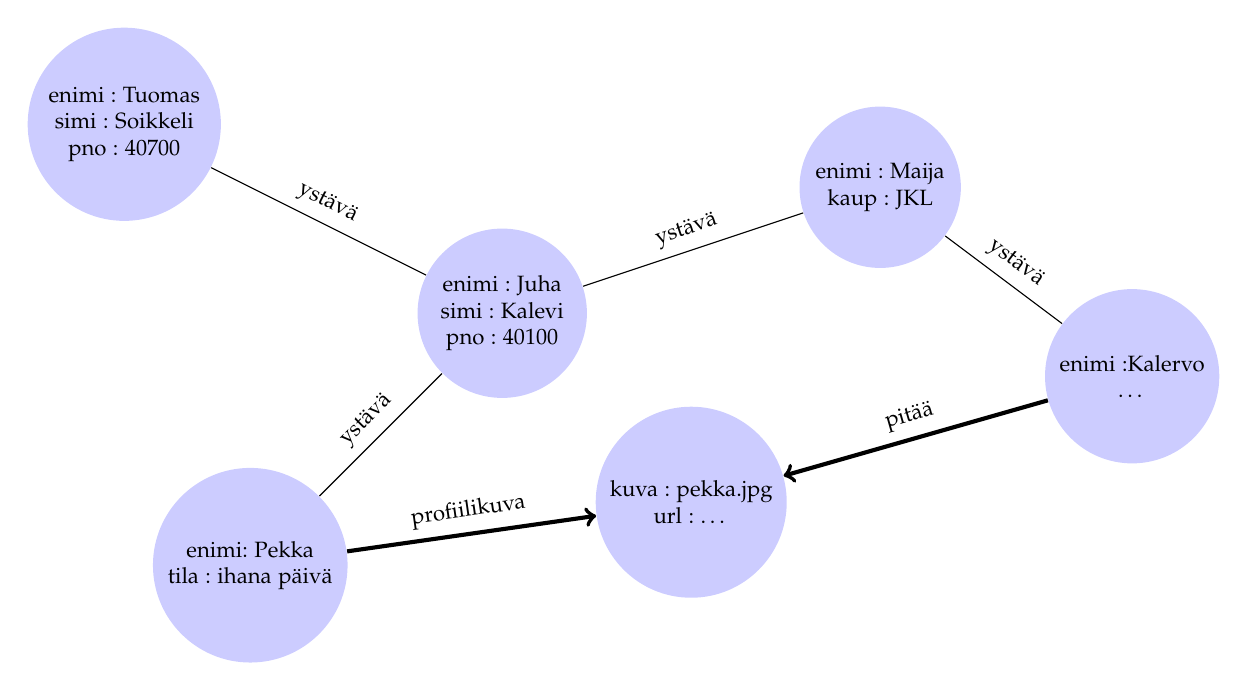
\begin{tikzpicture}[scale=.8,auto=left]
  
  \tikzstyle{every node}=[font=\footnotesize,align=center]
  \node[circle,fill=blue!20] (n6) at (0,10) 
    {enimi : Tuomas \\ simi : Soikkeli \\ pno : 40700};
  \node[circle,fill=blue!20,] (n4) at (6,7)
    {enimi : Juha \\ simi : Kalevi \\ pno : 40100};
  \node[circle,fill=blue!20,] (n5) at (12,9)  
    {enimi : Maija \\ kaup : JKL};
  \node[circle,fill=blue!20,] (n1) at (16,6) 
    {enimi :Kalervo \\ \ldots };
  \node[circle,fill=blue!20,] (n2) at (9,4)  
    {kuva : pekka.jpg \\ url : \ldots};
  \node[circle,fill=blue!20,] (n3) at (2,3)
    {enimi: Pekka \\ tila : ihana päivä};

  \foreach \from/\to in {n6/n4,n4/n5,n5/n1,n3/n4} 
    \draw (\from) -- (\to) node [midway, above, sloped] (TextNode) {ystävä};

  \draw[->,line width=1.5pt] (n1) -- (n2) node [midway, above, sloped] (TextNode) {pitää};
  \draw[->,line width=1.5pt] (n3) -- (n2) node [midway, above, sloped] (TextNode) {profiilikuva};
  
\end{tikzpicture}

\caption[VERKKOMALLI]{Esimerkki verkkoa käyttävästä tietomallista sosiaalisen median tietokantajärjestelmässä} 
\label{verkko}

\end{center}
\end{figure}

Verkkotietokannat sopivat sellaisiin tilanteisiin missä tieto on verkottunutta eli tieto paljolti relaatiossa. Tämä tarkoittaa että tietoalkiot liittyvät toisiinsa verkon kaaren avulla. Esimerkkejä verkkottuneesta tiedosta on sosiaalinen media, sisällönhallinta, suosittelujärjestelmät. Verkkotietokannat ovat hyödyllisiä myös tieteellisessä laskennassa. Jos tietokannan rakenteeseen kuuluu paljon monesta-moneen relaatioita, relaatiotietokannassa käytetään liitostauluja. Liitostaulut liitetään yhteen viiteavaimen avulla. Relaatiotietokannan useat liitokset (join) ovat raskaita, joita pyritään nopeuttamaan denormalisoimalla skeemaa. Verkkotietokannassa liitos on tavallinen operaatio. Jokainen verkon solu sisältää listan suhteistaan toisiin verkon soluihin. Nämä suhteet ovat järjestetty tyypin suunnan ja tyypin mukaan. Liitosta vastaava operaatio hakee tämän solun suhdetaulukosta lista, jolloin sillä on suora yhteys siihen liittyviin alkioihin. Tällöin tarve usean eri taulun läpikäyntiin häviää. Useita suhteita, eli verkon kaaria sisältävä skeema on myös helposti hajautettavissa ja koostettavissa MapReducen avulla.

Neo4j on Neo Technology -nimisen yrityksen valmistama avoimen lähdekoodin verkkotietokanta. Pääominaisuutena Neo4j:ssä katsotaan olevan ACID-ominaisuuksien noudattaminen. Neo4j tallettaa massivisen määrän dataa, mutta samalla takaa horisontaalisesti skaalattavissa ja tiedon jatkuvan saatavilla olon. Neo4j tarjoaa oman kyselykielen, jonka mainostetaan olevan tehokas ja luonnollista kieltä muistuttava kuten SQL-kieli. Hakuja on mahdollista tehdä myös REST-rajapinnan yli tai suoralla Java API:lla.


{\color{red}
\jyusection{YHTEENVETO}

NoSQL-tietokannat eroavat suuresti relaatiotietokannoista ja eivät noudata relaatiomallia.  NoSQL-tieto\-kannoista puuttuu tarkoituksellisesti tiettyjä relaatiotietokantojen ominaisuuksia, jotta saavutetaan tehokkuutta ja skaalautuvuutta. NoSQL-tieto\-kannat kuuluvat useisiin eri kategorioihin, joita on vaikea luokitella. Eri kategoiroiden NoSQL-tietokannoilla on moninaisia käyttötapauksia ja rajoitteita.

Avain-arvo-varastot keskittyvät tiedon tehokkaaseen käsittelyyn ja järjestelmän skaalautuvuuteen, ja usein ne tarjoavat vain rajallisen hakukielen tai -raja\-pinnan. Dokumenttivarastot ovat yleiskäyttöisempiä ja ne käyttävät hieman monimutkaisempia hakujärjestelmiä. Sarakepohjaiset tietokannat ovat suosittuja järjestelmiä tietovarastointiin ja analytiikkaan. Verkkotietokannat ovat verkkomallia käyttäviä tietokantoja, joihin tietoa voidaan tallentaa verkkoon. Tämä on luonnollinen malli tallentaa esimerkiksi sosiaalisen median dataa.

NoSQL-tietokantojen ominaispiirteitä ovat hajautettavuus, tehokkuus, yksinkertaisuus ja SQL-hakukielen puuttuminen. Näiden lisäksi NoSQL-tietokantojen oikeellisuumalli katsotaan olevan lähempänä BASE-ominaisuuksia kuin ACID-omi\-nai\-suuk\-sia, mutta poikkeuksia on runsaasti. 

\emph{Hajautettavuus} mahdollistaa tiedon käsittelyn kuluttajatason tietokoneissa, joten järjestelmää on helppo laajentaa ilman suuria kustannuksia. \emph{Tehokkuus} NoSQL-tietokannoissa johtuu käytettävästä oikeellisuusmallista, lopulta oikeellinen, joka mahdollistaa ACID-omi\-nai\-suuk\-sista luopumisen. ACID-ominaisuudet aiheuttavat suuria lisäkustannuksia tiedonkäsittelylle. NoSQL tietokantojen \emph{Yksinkertaisuus} johtuu siitä, että SQL-kielen katsotaan olevan monimutkainen hakukieli ja siitä luovuttaessa saavutetaan helpompia ja lyhyempiä, halvempia, järjestelmäkehityksen vaiheita. Toisaalta kehittäjät joutuvat toteuttamaan joitakin relaatiotietokantojen ominaisuuksia sovellustasolla, mikäli niitä tarvitaan. \emph{Hakurajapintana} käytetään tyypillisesti REST-rajapintaa HTTP-protokollan avulla. Tämän lisäksi yleisiä ovat ohjelmointikielen oma API, jolloin myöskin saavutetaan yksinkertaisuutta ja tehokkuutta, kun hakukielen kaltaisia välikäsiä ei ole.

NoSQL-tietokannat ovat saaneet osakseen huomattavan määrän kritiikkiä. Tutkittua tietoa on vähän johtuen teknologian nuoresta iästä, joten osa käyttäjäsegmentistä jättäytyy käyttämättä näitä teknologoita. Useat tutkijat ovat myös huomanneet, että NoSQL-tietokannat eivät ole vastaus kaikkiin tilanteisiin, vaan tietokanta tulee valita huolellisesti ja ei-relaatiotietokannat ovat yksi vaihtoehto muiden joukossa. Suuret yritykset kuten Google ja Amazon ovat valmistaneet omat järjestelmänsä käyttäen NoSQL-teknologoita, mutta se ei kerro, että kaikkien kehittäjien tulisi käyttää näitä tuotteita. Myöskän tehokkuus ei ole yksimielisesti NoSQL-tietokantojen ansiota. On argumentoitu ettei tehokkuus kärsi ACID-ominaisiuuksien toteuttamisesta vaan muista ominaisuuksista kuten esimerkiksi kirjanpidossa ja säikeiden hallinnassa. Uudet NewSQL-tietokannat tarjoavat relaatiotietokantojen ominaisuudet skaalattavassa ympäristössä, joten niiden kehittyessä esitetäänkin kysymys miksi enää käyttää NoSQL-tietokantoja.


%bibliography

\jyubibliography{viitteet}
}

%\attachmentsection{LIITE 1 ENSIMMÄINEN LIITE}
%\attachmentsection{LIITE 1 ENSIMMÄINEN LIITE}



\end{document}
